% Diapo d'intro
\begin{frame}
\frametitle{Contexte}

%introduire le développement des méthodes informatiques pour les systèmes complexes
%en particulier les systèmes biologiques dans le but de comprendre, modifier et 
%éventuellement contrôler le vivant. Ce qui implique donc de pouvoir 
% (1) Modéliser  (2) analyser (3) vérifier les comportements souhaités ou non.



%faire le lien entre modélisation, analyse et vérification des systèmes biologiques

%definition analyse: Étude minutieuse, précise faite pour dégager les éléments qui constituent un ensemble, pour l'expliquer, l'éclairer 

%definition vérification: vérifier si le modèle d'un système (souvent informatique ou électronique) satisfait une propriété. Par exemple, on souhaite vérifier qu'un programme ne se bloque pas, qu'une variable n'est jamais nulle, etc. 
\begin{tikzpicture}
 
 \uncover<2->{\node[auto] (sc) at (0,2) {Systèmes complexes};}
 \node[auto] (sb) at (0,1.5) {Systèmes \tval{bio}logiques};
 \only<1>{\node[esdef] (defsb) at (4,-5) {\begin{tabular}{c} Un système biologique est un ensemble d'organes/composants interagissant au \\ sein d'un organisme dans la réalisation d'une fonction biologique commune. \end{tabular}};}
\only<2>{\node[esdef] (defsc) at (4,-5) {\begin{tabular}{c} Systèmes complexes sont des réseaux des composants inter-agissants entre eux, \\ généralement de façon non déterministe. \end{tabular}};}

 
 
 \uncover<3->{\node[auto] (mi) at (7,1.5) {Méthodes \tval{informatiques}};
 
 \node[auto] (plus) at (3.5,1.5) {+};}
 
 \only<3>{\node[esdef] (defmi) at (4,-5) {\begin{tabular}{c} Méthodes informatiques: traitement automatique de l'information. \\\end{tabular}};}

 
 \uncover<4->{\node[es] (modeliser) at (0,-2) {Modéliser};}
 
 \only<4>{\node[esdef] (defmod) at (4,-5) {\begin{tabular}{c} Un modèle est une représentation simplifiée d'un système.\\ \end{tabular}};}

 
 \uncover<5->{\node[es] (analyser) at (3,-1) {Analyser};}
 
 \only<5>{\node[esdef] (defana) at (4,-5) {\begin{tabular}{c} Une analyse est une  étude minutieuse, précise faite pour comprendre\\ un système (modèle), pour l'expliquer, l'éclairer. \end{tabular}};}

 
 \uncover<6->{\node[es] (verifier) at (3,-3) {Vérifier};}

 \only<6>{\node[esdef] (defverif) at (4,-5) {\begin{tabular}{c} Une vérification (formelle) est le fait de prouver (de façon formelle)\\ la présence ou non d'une propriété dans un système. \end{tabular}};}

 
 
\uncover<7->{ 
\node (d1) at (4,-2) {};
\node (d2) at (6.5,-2) {};
 
 \draw[->,line width=6pt, color=lightgray] (d1) -- (d2) ;
 
 \node[auto] (butmodel) at (8,-2) {$
 \left\{
    \begin{array}{llll}
        Comprendre \\
        Prédire \\
        Modifier \\
        Contrôler
    \end{array}
\right.
$};
\begin{pgfonlayer}{background}
\draw[draw=blue!50, rounded corners=2mm, fill = white!20]
(-1.1, -3.4) rectangle (4.1, -0.5);
\end{pgfonlayer}
 }
 
 
\only<8>{\node[esdef] (but) at (4,-5) {\begin{tabular}{c}But: \tval{Développer les méthodes efficaces (complexité de calcul)}\\ \tval{pour l'analyse des grands modèles.}\end{tabular}};}
 \node[auto] (bp) at (4,-5.5) {};
%node[above=10pt,midway]{\textcolor{black}{\textbf{Algebraic Modelling}}} 
\end{tikzpicture}





\end{frame}




\begin{frame}[c]
  \frametitle{Contexte}
%rajouter le titre (version courte) dans toute les slides
\begin{center}
  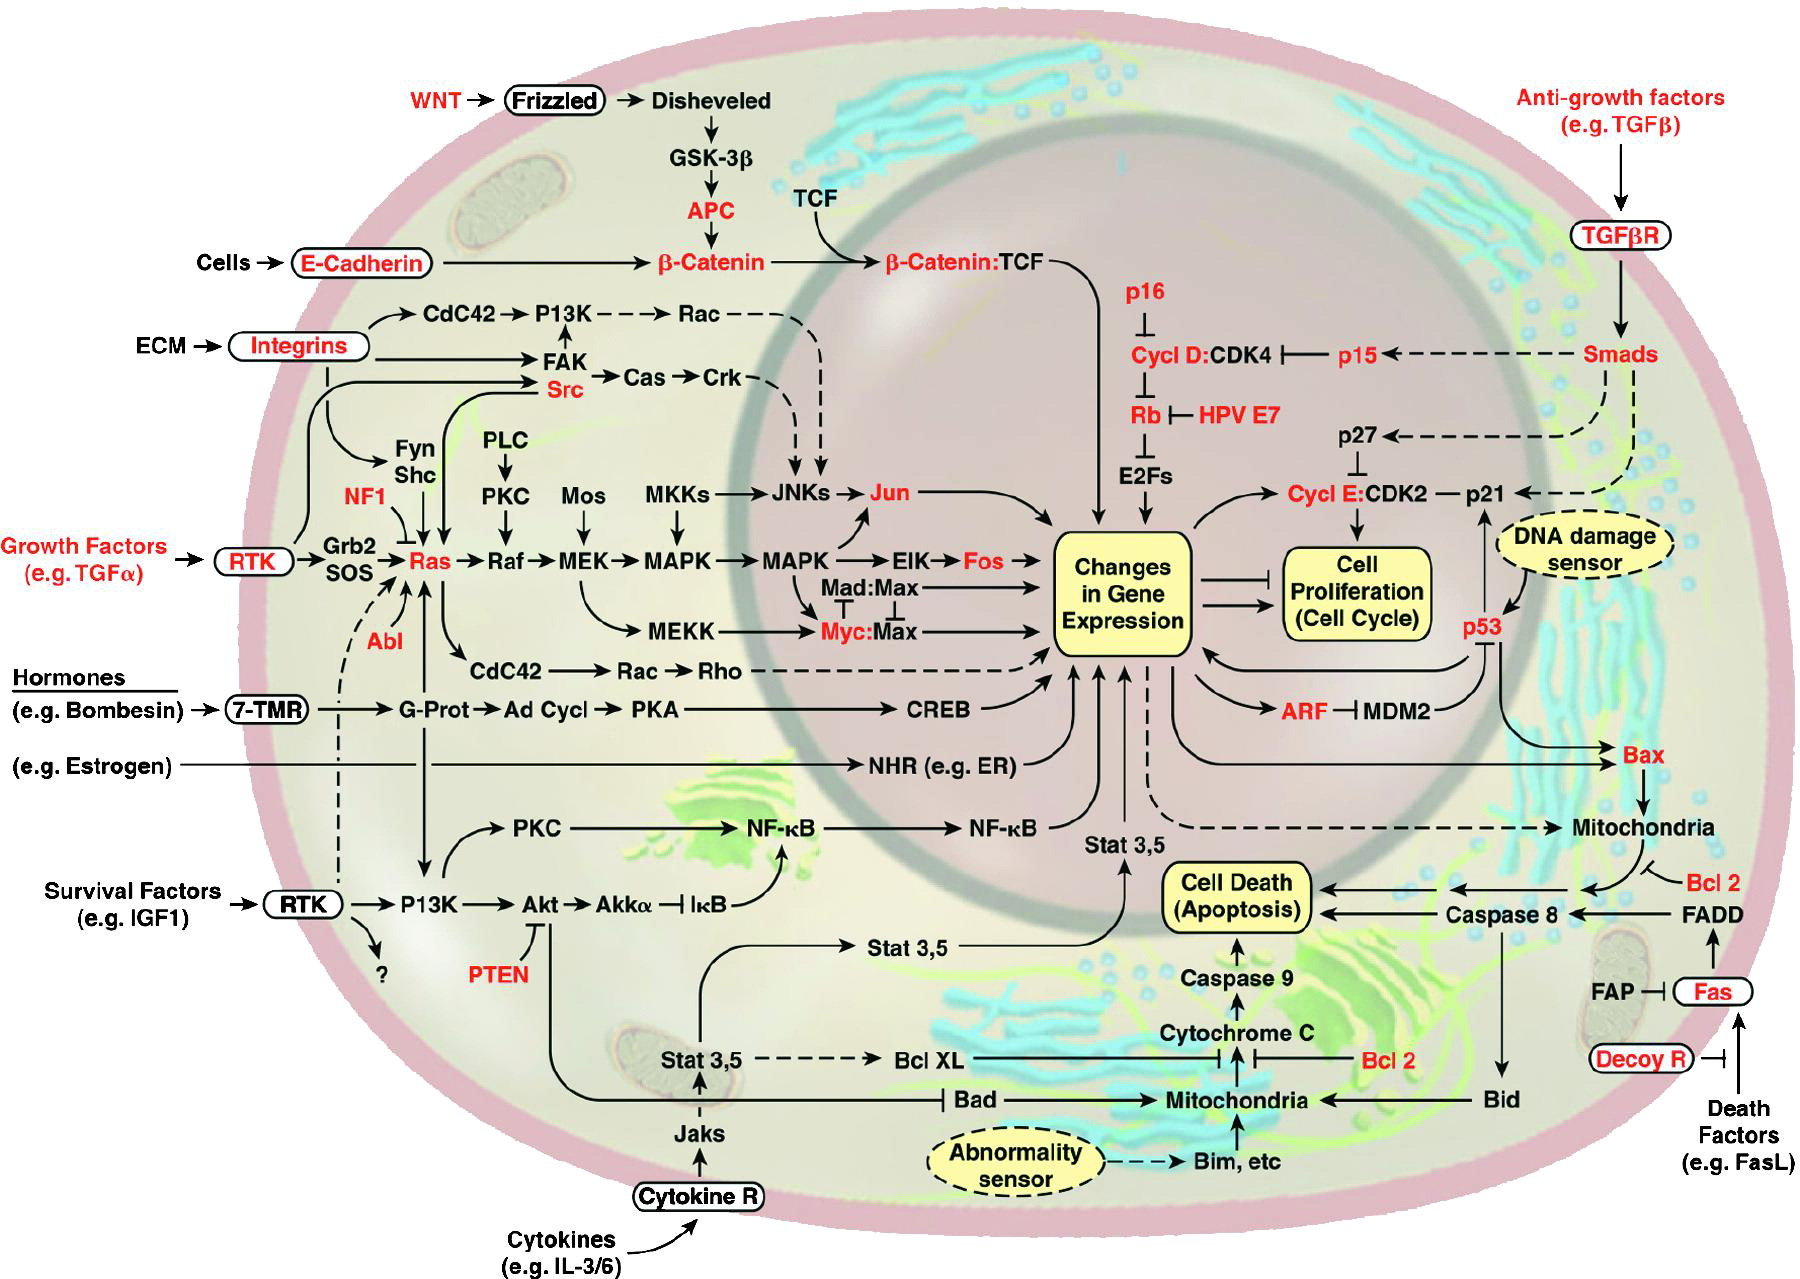
\includegraphics[scale=0.12]{images/cellule-description.jpeg}
\end{center}
\begin{center}
{\tiny \color{darkgreen}[\citelui]}
\end{center}

%\tcite{Wikipédia}

\begin{itemize}
%\item Cellular processes are driven by networks of biological interactions.
\item Processus cellulaire $\Longrightarrow$ des réseaux de régulation biologique (RRB).
\item N{\oe}uds (les composants biologiques), les arcs (les interactions).
%\item Proposer une modélisation formelle et une analyse des RRB.
%\item Formal modelling and analysis of Biological Regulatory Network.
%\item Static analysis of qualitative and quantitative properties.
\end{itemize}

%Cellular processes are driven by networks of biological reactions. Cells rely on the tight coordination of these pathways to achieve proper functioning.
%With the help of signaling pathway, a cell senses changes in its environnement or internal state. This information is then passed on via cascades of biochemical 
%reactions to the appropriate mechanisms which respond by modifying the metabolic and transcriptiona activities. this in turn modifies the behavior of the cell.

%Consequently, the dynamics of biopathways play a crucial role in determinig cellular functions.

%Examples: circadian rhythm, the apoptosis pathway inducing programmed cell death, cell differentiation.

%\textcolor{couleurtheme}{$\Rightarrow$} \fbox{\tval{\large The need of comprehension of biological systems}} \textcolor{couleurtheme}{$\Leftarrow$}


%\textcolor{couleurtheme}{$\Rightarrow$} \fbox{\tval{\large Allow efficient translation from Process Hitting to BRN}} \textcolor{couleurtheme}{$\Leftarrow$}

\end{frame}


